\documentclass[11pt]{article}
\newcommand{\tablelang}{en}
% Shared preamble for paper/tex/en/main.tex and paper/tex/uk/main.tex (XeLaTeX via Tectonic).
% Same layout as the author's earlier preprint (Zenodo 23375871): A4, 25 mm, CMU fonts, natbib numbers.
\usepackage[a4paper,margin=25mm]{geometry}
\usepackage{fontspec}
\setmainfont{cmunrm.otf}[BoldFont=cmunbx.otf,ItalicFont=cmunti.otf,BoldItalicFont=cmunbi.otf]
\setsansfont{cmunss.otf}[BoldFont=cmunsx.otf,ItalicFont=cmunsi.otf]
\setmonofont{cmuntt.otf}[BoldFont=cmuntb.otf,ItalicFont=cmunit.otf]
\usepackage[ukrainian,english]{babel}
\usepackage{amsmath,amssymb}
\usepackage{booktabs,tabularx,array,longtable}
\usepackage{graphicx}
\usepackage[font=small,labelfont=bf]{caption}
\usepackage{xcolor}
\usepackage{microtype}
\usepackage[numbers,sort&compress]{natbib}
\PassOptionsToPackage{hyphens}{url}
\usepackage[hidelinks]{hyperref}
\usepackage[nameinlink,capitalise,noabbrev]{cleveref}
\usepackage{url}

\graphicspath{{../../figures/}}
% primitive input: LaTeX's \input is not expandable and breaks inside tabular after \midrule
\makeatletter\newcommand{\gentable}[1]{\@@input ../tables/\tablelang/T#1.tex }\makeatother
\newcommand{\code}[1]{\texttt{#1}}
\newcolumntype{L}{>{\raggedright\arraybackslash}X}
\newcolumntype{R}{>{\raggedleft\arraybackslash}p{1.1cm}}
\definecolor{lvA}{HTML}{2a78d6}\definecolor{lvB}{HTML}{eb6834}\definecolor{lvC}{HTML}{1baf7a}\definecolor{lvD}{HTML}{eda100}
\setlength{\tabcolsep}{4pt}
\renewcommand{\arraystretch}{1.12}
\setlength{\emergencystretch}{2em}
\sloppy

\hypersetup{pdftitle={Low-cost coding agents in survival Minecraft},pdfauthor={Oleksandr Pylypenko}}

\begin{document}
\selectlanguage{english}

\title{Low-cost coding agents in survival Minecraft: a tested skill library, a twelve-day run of four Gemini~3.8~Flash agents, and a server-log audit of every milestone}
\author{Oleksandr Pylypenko\\[2pt]\small ORCID: \href{https://orcid.org/0009-0004-9610-9242}{0009-0004-9610-9242}}
\date{2026-11-02 \quad (v1.0)}
\maketitle

\begin{abstract}
\noindent
We partially reproduce the setting of arXiv:2610.22319, in which four Gemini~4~Argon agents beat Minecraft by writing JavaScript programs for the Mineflayer library. Our setting differs in a cheaper model (Gemini~3.8 Flash High through the Antigravity CLI), a limited token budget, and a tested skill library given to the agents at the start: 54 functions, among them a recursive \code{lib.obtain(item, n)} that derives the whole chain of prerequisites from the game data. We describe the infrastructure (a sandboxed bridge, a turn watchdog, ``parking'' of idle bots, a cutaway viewer), 20 defects found while testing it, two pilot runs and a main run of 294 calendar hours, 20.1 of them active play. In that time 2--4 agents ran 3770 programs (21.2\,\% failed; 70.4\,\% of the failures were time-outs) and died 332 times. The main contribution is the audit: each of 16 milestones receives an evidence level A--D by a mechanical rule over the server log. Level A means that no console command at all preceded the milestone. The agents completed stage~1 (stone, iron, armour, bed, diamonds, diamond pickaxe, flint and steel, obsidian) at level~A in 2.4 active hours. Entering the Nether, finding a fortress and the first blaze rod are level~B (the only help was night skipping), but by then the agents were using helpers that the operator's supervising session had added during the run (mark +K). Ender pearls and eyes of ender are level~C (permanent status effects, enchantments, \code{keepInventory}). We do not credit the agents with the stronghold, the End or the dragon: console commands produced those milestones (teleports, \code{/fill} of the portal, \code{/damage} to the dragon, an advancement grant), level~D. Fire, ghast fireballs and lava account for 63.6\,\% of deaths. The model used 13\,652 steps, 50.8\,M uncached input tokens (1922.9\,M more from the cache, 97.4\,\%), 8.82\,M output and 4.06\,M reasoning tokens.
\end{abstract}

\noindent\textbf{Keywords:} LLM agents; multi-agent systems; Minecraft; Mineflayer; skill library; long horizon; audit; reproducibility.

\medskip
\noindent\textbf{Independence statement.} This is an independent partial reproduction of the setting of arXiv:2610.22319 (Google DeepMind). As of 2026-11-02 there was no contact with its authors; the work was not coordinated with or reviewed by them. We do not use Gemini~4~Argon and do not claim our results are directly comparable to theirs.

\smallskip
\noindent\textbf{Use of AI.} The infrastructure, skill library, agent guides, analysis scripts and a draft of this text were produced in Claude Code sessions (Claude Opus~5.5, Anthropic) directed by the author. The players were driven by Gemini~3.8 Flash High agents in the Antigravity CLI (\code{agy}). A separate \code{agy} session (the \emph{supervising session}) carried out the author's requests during the run: it started and stopped the game, edited the agents' instructions and helpers and, at the author's request, issued server console commands. The README illustration was generated by a Gemini image model. Every number in this paper is reproduced by \code{paper/scripts/run\_all.sh} on the published data.

\section{Introduction and motivation}
In arXiv:2610.22319~\citep{faldor2026} four Gemini~4~Argon agents went from bare hands to defeating the Ender Dragon in 27\,h\,14\,min, running 2783 programs and dying 605 times. They had no game-specific tools: only Mineflayer~\citep{mineflayer}, its path-finding plugin and a one-paragraph goal. The authors estimate the run at about \$520 at introductory list prices.

At the other end, Odyssey~\citep{odyssey} gives agents a large skill library (40 primitive and 183 compositional skills), which lets even an 8-billion-parameter model solve tasks such as ``obtain a diamond''; without the library, in the authors' ablation, such a model hardly produces executable code. Voyager~\citep{voyager} grows its own library with GPT-4.

We asked an intermediate question: how far do cheaper coding agents get when they receive a tested skill library and guides but keep full freedom of code and coordination, and how should one report a run into which the operator stepped under budget pressure? The second question turned out to matter as much as the first: near the end of our run, the operator's supervising session ``finished'' the game with console commands at the author's request, and without an audit against the server log this part would read as the agents' result.

\section{What is checked and what is out of scope}
\textbf{Checked:} how far along the Minecraft technology tree 2--4 Gemini~3.8 Flash High agents with a skill library, a watchdog and guides get, and in how much active time; which failures (deaths, program errors, infrastructure defects) set the pace; whether what the agents achieved can be separated, mechanically and from the server log, from what operator commands did.

\textbf{Out of scope:} a controlled comparison of models (one run, one model); a dragon kill by the agents (not achieved, \cref{sec:milestones}); playing from pixels (agents see the world only through the Mineflayer API); judging the guides separately from the library (they changed together).

\section{Contributions, and what they do not claim}
\begin{enumerate}\renewcommand{\labelenumi}{(\alph{enumi})}
\item \textbf{Open infrastructure}: a bridge to Mineflayer with a \code{vm} sandbox and an allow-list of modules, the \code{./mc} command for agents, a turn watchdog for \code{agy}, parking of idle bots, protection of placed blocks from the path finder, an overhead cutaway viewer. \emph{Not claimed:} that it is optimal or works unchanged on other game versions.
\item \textbf{A skill library} of 54 functions, including \code{lib.obtain}, which derives the chain of prerequisites from game data (recipes, block drops, harvest tools, smelting, mob drops). Every skill was tested on the server; the defects found are listed in \cref{tab:defects}. \emph{Not claimed:} completeness; combat, the Nether and the End are covered weakly.
\item \textbf{Results} of two pilots and a main run, with evidence levels A--D for 16 milestones (\cref{tab:milestones}). \emph{Not claimed:} that the agents beat the game; milestones M14--M16 are level~D.
\item \textbf{An audit method}: a mechanical rule over the server log, and a separate +K mark for helpers the operator added during the run. \emph{Not claimed:} that it detects every form of help; it sees changes to the instructions and advice only through the agents' use of helpers.
\item \textbf{A failure analysis}: 332 deaths by cause and phase, 798 failed programs by class. \emph{Not claimed:} a causal link between assistance phase and death rate; the phases coincide with the move into the Nether.
\item \textbf{Token accounting} for the main run. \emph{Not claimed:} a monetary cost; quota access through Antigravity has no transparent per-token price.
\end{enumerate}

\section{Environment and agents}
\paragraph{Server.} Vanilla Minecraft Java Edition 1.20.1 in Docker (\code{itzg/minecraft-server}), survival, Easy, no cheats, command blocks or RCON; the only operator is the human spectator. We started on 1.20.4, as arXiv:2610.22319 did, but moved to 1.20.1 because the 3D viewer prismarine-viewer ships the block-state palette of exactly that version and drew underground blocks wrongly on 1.20.4 (defect D12).

\paragraph{Bridge.} Each player has its own Node.js process with a Mineflayer bot. An agent writes a program to a file and runs \code{./mc run file --timeout N}. The program runs as the body of an \code{async} function in a \code{vm} sandbox; its globals are \code{bot}, \code{lib}, \code{console}, \code{isCancelled()}, \code{Vec3}, \code{mcData}, \code{goals}, \code{Movements}, \code{sleep}. Only the Mineflayer packages and a few harmless Node modules can be required; processes, files and the network are unavailable. Values on \code{globalThis} persist between programs, and the team's and the agent's \code{autoload.js} run after every bridge start. After a time-out \code{isCancelled()} becomes true and movement and digging stop. The output of a program is followed by position, health, food, phase of day, nearby hostiles, tool durability and new chat. After 5 minutes without programs the bot logs out (``parking'') and comes back with the next program; chat and events meanwhile are read from the server log.

\paragraph{Skill library.} 54 functions (\code{bridge/lib/skills.js} and \code{obtain.js}, 1442 lines at the end of the run): looking around, movement (digging allowed, but never through blocks the agents placed), gathering, crafting with recovery from failures, placing and blueprints (house, portal frame), chests, smelting, combat, shelter, sleep, a staircase down to diamonds, buckets, obsidian from lava and water, doors. In tests from an empty inventory an iron pickaxe took 96\,s, a bucket 99\,s and full iron armour about 6\,min.

\paragraph{How \code{lib.obtain} derives a chain.} \code{lib.obtain(item, n)} makes sure at least \(n\) items are in the inventory and for each missing item picks a source in this order. (1) Smelting, if the item is in the smelting table (ingots, glass, cooked meat, charcoal): first the input, then fuel at 8 items per coal or 1.5 per plank or log, and only right before smelting it finds or places a furnace. (2) Crafting: among all recipes the cheapest by an estimate of ingredient cost is chosen; recipes that consume storage blocks are dropped and recipes from the same item family (a bed from a bed) get a penalty of 5000 to avoid recolouring loops. The crafting table is made first, since otherwise it eats the planks gathered for the recipe; ingredients are gathered in several passes until all are in the inventory at once. (3) Hunting for mob drops (leather, wool, string, pearls). (4) Mining: source blocks come from the game data (\code{drops}), the tool from \code{harvestTools}; a missing tool is obtained recursively. For deep ores not in reach it first digs a staircase down to the ore's usual level (diamonds \(-54\)) with three spare stone pickaxes, and if the stairs run into liquid it walks about 28 blocks away and starts again. Obsidian, rarely lying around, is made: water is poured onto the edge of a lava pool and the result is mined with a diamond pickaxe. Every step is logged and returned to the agent; if the player dies, the skill stops at once and reports where the items lie.

\paragraph{Instructions.} \code{AGENTS.md} (goal, golden rules, how to play, memory) and seven guides (library, survival, programs and errors, recipes, building, teamwork, iron age): 7452 words in all. The guides were written from the pilots and tests; every piece of code in them was run on the server.

\paragraph{Agents.} Each player is driven by its own Gemini~3.8 Flash High agent in the Antigravity CLI with all tools allowed. A watchdog (\code{agent-loop.sh}) runs turn after turn in the same conversation and adds the player's current status after each turn. Until 24~October two agents played (alpha, beta), then four (gamma and delta joined at 17:22 UTC). The instructions state the Ender Dragon as the long-term goal and the current stage as numbered milestones.

\paragraph{Viewer.} For watching we wrote a camera that follows the player from above, shows a cutaway underground (blocks above the player are not drawn) and darkens the sky with the game time (D13, D14). Agents do not see the viewer.

\section{Audit method}\label{sec:method}
The source of truth is the Minecraft server log. \code{extract.py} parses every log file into a table of events: advancements, deaths, joins and leaves, chat, and the feedback of console commands. Lines such as ``Teleported \dots'', ``Applied effect \dots'' or ``Successfully filled \dots'' carry no player name; since the human spectator is the only operator, they come from the server console, which the supervising session used through \code{docker exec}.

The level of a milestone depends on the commands that appeared in the main run before it:
\textcolor{lvA}{\textbf{A}}~no console command at all;
\textcolor{lvB}{\textbf{B}}~only time changes and the \code{playersSleepingPercentage} rule (night skipping), and read-only queries;
\textcolor{lvC}{\textbf{C}}~assistance was active: status effects, enchantments, game rules (\code{keepInventory}), item gifts, block fills;
\textcolor{lvD}{\textbf{D}}~a teleport, damage, entity kill, item gift or advancement grant within 15 minutes before the milestone.
Separately, \textbf{+K} counts the helpers the supervising session added to \code{team/autoload.js} during the run that the agents had already called (last column of \cref{tab:milestones}); first use is taken from the program code. We could not attribute the definition of any of these helpers to a write by the agents themselves.

The main run starts at 2026-10-21 12:11 UTC, when the agents were launched. Programs at 12:06--12:10 were our library tests on the same player alpha and gave alpha a stone and an iron pickaxe before the start (\cref{sec:limits}); milestones M01 and M02 are therefore credited to beta, which reached them on its own.

\textbf{Coverage.} 3766 of the 3770 programs of the main run fall into stretches covered by the server log; the other 4 fall into seconds of server shutdown. The server log of 21~October 00:00--11:59 UTC is missing (rotation over restarts); this affects only the idle night after pilot~2, which we count from the bridge's chat log.

\textbf{Active time} is the union of program intervals of all agents, with gaps up to 5 minutes counted as play (the agent thinking); longer pauses (quota, stops) are excluded.

\section{Results}
\subsection{Pilots}
Pilot~1: two agents without guides or library, goal ``build a structure''. In 15 minutes: 8 deaths at night (34.9 per active hour) and about 20 wall blocks, after which the author stopped the run. Pilot~2, with guides and the first library: 2 deaths in active play, a 5\(\times\)5 sandstone house (89 blocks, checked independently by both agents with \code{lib.materials}), and agents that declared ``100\,\% COMPLETE'' and ended their turns. The bots then stood without agents for 8.2 hours of night and died 42 times; about 60 of the 89 house blocks were left, most likely after creeper explosions. These two observations produced the turn watchdog (D15) and parking (D16).

\begin{table}[h]\centering\small
\caption{Runs. Active hours: union of program intervals, gaps up to 5 min. lib\,\%: share of programs calling the skill library.}\label{tab:runs}
\begin{tabularx}{\linewidth}{@{}L rrrrrrr@{}}\toprule
run & agents & wall h & active h & programs & errors \% & deaths & lib \% \\\midrule
\gentable{1}\bottomrule\end{tabularx}
\end{table}

\subsection{Main run: milestones}\label{sec:milestones}
\Cref{tab:milestones} and \cref{fig:timeline}. The agents completed stage~1 at level~A with no operator helpers: beta made the first stone tools 2 minutes after the start, diamonds and a diamond pickaxe after 2.0--2.1 active hours, obsidian (water on lava) after 2.4. Entering the Nether (delta, 7.4 active hours), the fortress (delta, 9.6) and the first blaze rod (gamma, 13.4) are level~B, i.e.\ without console help apart from night skipping, but with +K: the agents were already using operator helpers, among them \code{makeObsidianSafe} for the portal obsidian and \code{configureFireAvoidance} for walking around fire. Ender pearls and an eye of ender (beta, 18.9 and 19.1) are level~C: permanent effects (Haste~III, Resistance, Fire Resistance, Speed, Saturation), Looting~III and \code{keepInventory} were active. We do not credit the agents with the stronghold portal room, entering the End and the dragon's death within 5 minutes (18:01--18:06 UTC on 2~November): the supervising session found the stronghold by reading the world's region files, filled the portal with \code{end\_portal} blocks, teleported the players, killed the crystals, damaged the dragon with \code{/damage} and granted the advancement with \code{/advancement}: level~D.

\begin{table}[h]\centering\small
\caption{Milestones of the main run: first time any agent reached each, with evidence level and the number of operator-added helpers already in use (+K).}\label{tab:milestones}
\begin{tabularx}{\linewidth}{@{}l L l l r r c r@{}}\toprule
id & milestone & first (UTC) & agent & wall h & active h & level & op.\ helpers \\\midrule
\gentable{2}\bottomrule\end{tabularx}
\end{table}

\begin{figure}[h]\centering
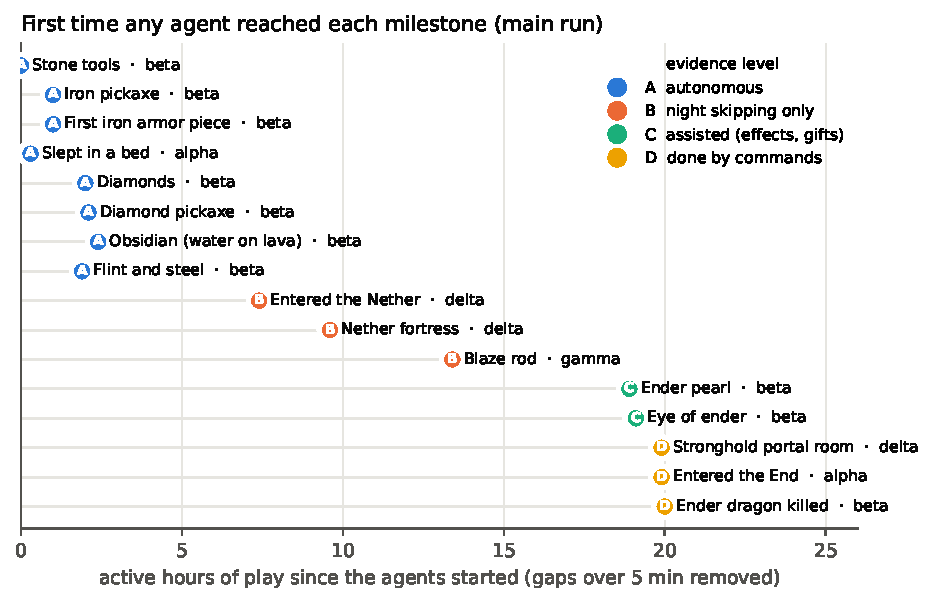
\includegraphics[width=\linewidth]{F1_timeline.pdf}
\caption{First time any agent reached each milestone, over active hours; colour and letter give the evidence level.}\label{fig:timeline}
\end{figure}

\subsection{Interventions}
\Cref{tab:commands} and \cref{fig:activity}. Phase~A had no console commands. Phase~B (from 23~October) had only 59 time and sleep commands (\code{time set}, \code{playersSleepingPercentage}) and 8 experience queries. Phase~C began on 1~November at 17:00 UTC: after the author asked for ``all improvements'' (31~October), the supervising session extended \code{auto-skip-night.sh}, which switched on \code{keepInventory}, effects and enchantments through the console. The author started phase~D on 2~November at 17:59 with the words ``this is no longer the agents' work, it is dumb farming \dots\ help them as much as possible''. Phase~C held 702 block fills (mostly rebuilding the portal frame every 15\,s), 55 effects, 26 enchantments, 20 game rules, 15 spawn points and 2 item gifts. Phase~D lasted 12 minutes: 15 teleports, 100 fills (End portal, walkways in the End), 5 damage commands, 1 entity kill, 3 item gifts and 2 advancement grants; 1071 console commands in all.

\begin{table}[h]\centering\small
\caption{Console commands of the main run by family and phase.}\label{tab:commands}
\begin{tabular}{@{}l rrrrr@{}}\toprule
family & A & B & C & D & total \\\midrule
\gentable{3}\bottomrule\end{tabular}
\end{table}

\begin{figure}[h]\centering
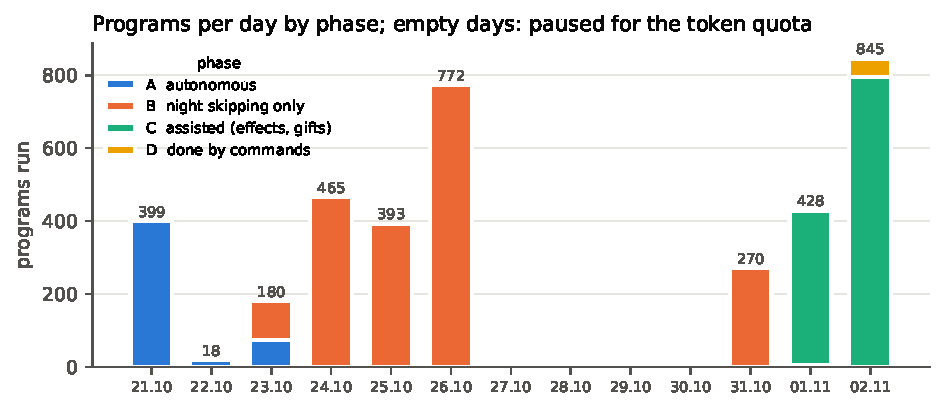
\includegraphics[width=\linewidth]{F3_activity.pdf}
\caption{Programs per day by phase. Days without bars: the game was paused for the token quota.}\label{fig:activity}
\end{figure}

\subsection{Deaths}
\Cref{tab:deaths}, \cref{fig:deaths,fig:deathrate}. Of the 332 deaths of the main run 211 (63.6\,\%) were fire, ghast fireballs and lava, i.e.\ the Nether. Phase~A had 11 deaths in 4.5 active hours (2.4 per hour, mostly drowning), phase~B 17.7 per hour, phase~C 25.1. The rise coincides with the move into the Nether, not only with the assistance phase; even with Fire Resistance phase~C produced 48 fire deaths as the agents walked carelessly over soul sand and near lava.

\begin{table}[h]\centering\small
\caption{Deaths of the main run by cause and phase.}\label{tab:deaths}
\begin{tabular}{@{}l rrrrr@{}}\toprule
cause & A & B & C & D & total \\\midrule
\gentable{4}\bottomrule\end{tabular}
\end{table}

\begin{figure}[h]\centering
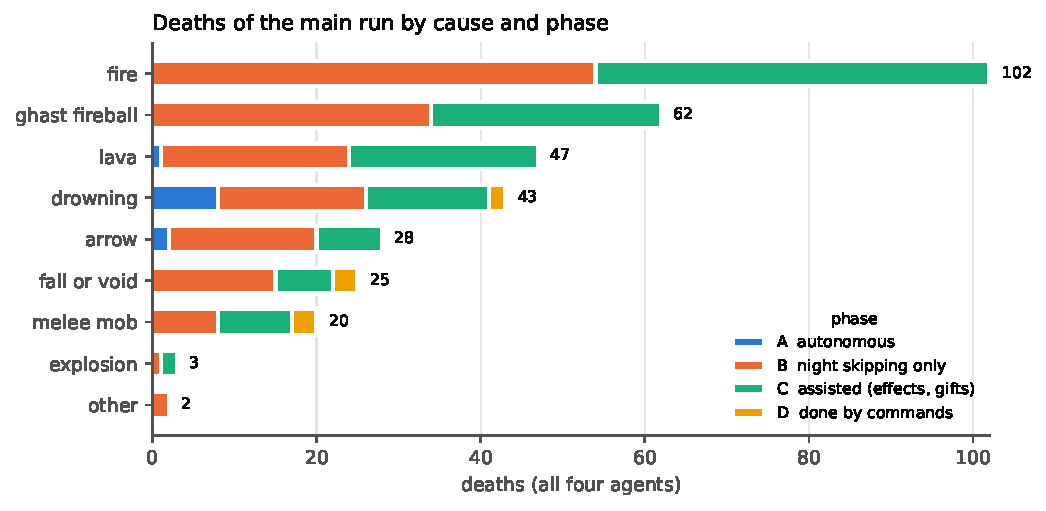
\includegraphics[width=\linewidth]{F2_deaths.pdf}
\caption{Deaths of the main run by cause, stacked by phase.}\label{fig:deaths}
\end{figure}

\begin{figure}[h]\centering
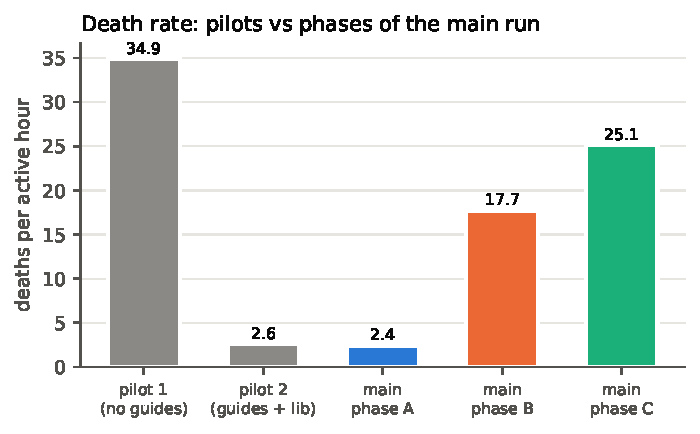
\includegraphics[width=0.72\linewidth]{F4_death_rate.pdf}
\caption{Deaths per active hour in the pilots and the phases of the main run (phase D lasted 12 minutes and is left out).}\label{fig:deathrate}
\end{figure}

\subsection{Program errors}
\Cref{tab:errors}. 798 of 3770 programs (21.2\,\%) failed; 70.4\,\% of the failures were time-outs, where the agent chose too short a time for a long action (mining, a march in the Nether). Errors in the code itself (TypeError, ReferenceError) are only 4.0\,\% of failed programs: the model writes JavaScript confidently; its weak point is judging how long actions and situations in the world take.

\begin{table}[h]\centering\small
\caption{Failed programs of the main run by error class.}\label{tab:errors}
\begin{tabular}{@{}l rr@{}}\toprule
class & programs & \% of failed \\\midrule
\gentable{5}\bottomrule\end{tabular}
\end{table}

\subsection{Agents and cost}
\Cref{tab:agents}. The median program runs 8.8\,s. The share of programs calling \code{lib.obtain} is small (1.2--3.7\,\%) because the agents wrapped it in their own helpers; 92.6\,\% of programs use the library in some way. Tokens were counted from each agent's own stream (a model step is one response or tool call): 13\,652 steps, 50.8\,M uncached input tokens, 1922.9\,M cached (97.4\,\%), 8.82\,M output and 4.06\,M reasoning tokens. The Antigravity quota forced pauses: from 27 to 30~October the game did not run at all (\cref{fig:activity}).

\begin{table}[h]\centering\footnotesize
\caption{Agents of the main run. Token columns in millions; \emph{cached} input was served from the context cache.}\label{tab:agents}
\setlength{\tabcolsep}{3pt}
\begin{tabular}{@{}l l rrrrrrrrrr@{}}\toprule
agent & first program & progr. & err.\,\% & med.\,s & obtain\,\% & deaths & steps & input & cached & output & think \\\midrule
\gentable{6}\bottomrule\end{tabular}
\end{table}

\subsection{Infrastructure defects}
\Cref{tab:defects} lists twenty defects found while testing the skills and during the run. Some of them the agents would hardly have worked around on their own, since they lie in Mineflayer, its plugins or the viewer: a stack left on the cursor after a failed craft (D01), the path finder breaking walls (D03), doors it cannot pass (D04), air reported in ticks instead of bubbles (D11), mismatched palettes (D12). We consider this table a practical result in its own right for anyone building agents on Mineflayer.

\begin{table}[h]\centering\footnotesize
\caption{Defects of the infrastructure found during testing and the run.}\label{tab:defects}
\begin{tabularx}{\linewidth}{@{}l l L L l@{}}\toprule
id & area & symptom & fix & found in \\\midrule
\gentable{7}\bottomrule\end{tabularx}
\end{table}

\subsection{Agent behaviour}
We did not read all 3770 programs; below are episodes we watched live, each findable in the chat logs (UTC).
\begin{itemize}
\item \emph{Agreement and self-organisation.} In pilot~1, 30 seconds after the start, beta proposed a wooden cabin and alpha agreed and named the site (19:00:57--19:01:27). In pilot~2 the proposals crossed: alpha accepted beta's plan (7\(\times\)7) while beta accepted alpha's (5\(\times\)5) (19:57:20--19:57:29); the agents noticed and settled on one site.
\item \emph{Adaptation.} Pilot~2 started in a desert with no tree within 128 blocks. The guides said nothing about sand; the agents decided to build from sandstone crafted from sand, and beta worked out the block budget of a 5\(\times\)5 blueprint (20:04:43--20:07:52).
\item \emph{Care for the teammate.} ``Beta: Skeleton in the pit at (36, 75, -19)! Stay above Y=78'' (19:10:05, pilot~1); ``Recovering items from creeper blast!'' (19:08:58); in the main run, after alpha drowned, beta reported that the bed and spawn point were set and food and tools left in the chest, and asked where alpha's items were (21~October, 12:33:23).
\item \emph{Night protocol.} The agents waited out nights inside the base with long waiting programs (e.g.\ 21~October 12:17--12:35), as the guide asks, instead of working outdoors.
\item \emph{Ending the turn.} In pilot~2 both agents, having got ``100\,\% COMPLETE'' from \code{lib.materials}, wrote a summary and ended their turns although the instructions said to keep going; this is why the watchdog exists.
\item \emph{Reporting.} In phase~C the agents repeated the same milestone in chat many times (``MILESTONE 8 100\% COMPLETE!'', 1~November 18:56--18:57, several agents in a row). At the end of the run the team notes contained the supervising session's entries about the stronghold and the dragon, which we do not credit to the agents.
\end{itemize}

\section{Comparison with earlier work}
arXiv:2610.22319~\citep{faldor2026}: four Gemini~4~Argon agents, no library, 27\,h\,14\,min of continuous play, 605 deaths, dragon killed by the agents. Our run: 2--4 Gemini~3.8 Flash High agents with a library, 20.1 active hours over 12 days with quota pauses, 332 deaths; autonomous (A) only stage~1, the Nether up to the blaze rod at B with +K. Differences in model, budget and continuity do not allow attributing the gap to any one cause.

Odyssey~\citep{odyssey}: a library of 223 skills, tasks up to diamonds and single fights; the library alone obtains a diamond within 10 minutes in 92.5\,\% of attempts. Our \code{lib.obtain} derives the chain for any item from the game data instead of 183 hand-written skills; the agents reached a diamond pickaxe in 2.1 active hours, but unlike Odyssey we have one run, not a series.

\section{Limitations and threats to validity}\label{sec:limits}
\paragraph{One run.} All numbers come from one main run and two short pilots; the spread is unknown.
\paragraph{Alpha's head start.} Our library tests at 12:06--12:10 gave alpha a stone and an iron pickaxe before the agents started. M01 and M02 are credited to beta, but the tools in the team may have sped up the early game.
\paragraph{Operator in the loop.} During the run the supervising \code{agy} session changed \code{team/autoload.js} 10 times, the instruction template 7 times, \code{skills.js} 5 times, and the guides; these changes contained coordinates (blaze spawner, portal) and ready-made helpers. The +K mark reflects only helpers the agents called in code; it does not see advice in the instruction text.
\paragraph{Night skipping.} We treat level~B as nearly autonomous because skipping the night is equivalent to sleeping in a bed. But \code{playersSleepingPercentage = 1} and \code{time set} need no bed and so make the game easier than sleeping does.
\paragraph{Hidden help.} From 1~November (19:24 UTC) the \code{logAdminCommands} rule was switched off and on 14 times; while it is off, commands an operator types in the game are not logged, while console commands still are. The human operator joined four times as a spectator; no command of theirs appears in the log.
\paragraph{Missing data.} The server log of 21~October 00:00--11:59 UTC is missing; the idle night of pilot~2 is counted from the bridge log (42 deaths).
\paragraph{Changing library.} \code{skills.js} and the guides changed during the run; versions are not pinned per milestone. We publish the repository state and its git history.
\paragraph{Model and access.} Gemini~3.8 Flash High through Antigravity with a quota; other models were not tried. Token accounting for the pilots is missing.
\paragraph{Perception through an API.} Mineflayer gives agents exact coordinates of blocks and entities, also behind walls; a human player has no such information.

\section{Data and code availability}
Code of the infrastructure, library, guides and analysis: \url{https://github.com/cyberdid/minecraft-ai-agents} (MIT). Raw data: bridge logs and \code{agy} streams (\code{logs/}), pilot archives (\code{runs/}), the server log (\code{paper/data/raw/server-logs/}), saved worlds (\code{server/saves/}, including \code{stage1-complete-4agents-portal-lit}). All tables and figures are rebuilt by \code{bash paper/scripts/run\_all.sh}, which lists every input with its SHA-256 (\code{paper/data/derived/manifest.csv}), checks the tables of the master text and builds the PDFs.

\section{History of revisions}
v1.0 (2026-11-02): first version. While preparing it we corrected our own analysis errors: (1) the main run was first taken to start at the first program (12:06), which wrongly credited M01--M02 to alpha on the basis of our tests; (2) the archived pilot logs contained our library tests, so pilot~1 first showed 17 deaths instead of 8; (3) \code{gamerule playersSleepingPercentage} was first classified as assistance (level~C) instead of night skipping (B).

\begin{thebibliography}{9}
\bibitem{faldor2026} M.~Faldor, S.~Singh, R.~Raileanu. A team of Gemini 4 Argon agents beats Minecraft. arXiv:2610.22319, 2026.
\bibitem{odyssey} S.~Liu et al. Odyssey: Empowering Minecraft Agents with Open-World Skills. arXiv:2407.15325 (v3), 2025.
\bibitem{voyager} G.~Wang et al. Voyager: An Open-Ended Embodied Agent with Large Language Models. TMLR, 2024. arXiv:2305.16291.
\bibitem{minedojo} L.~Fan et al. MineDojo: Building Open-Ended Embodied Agents with Internet-Scale Knowledge. NeurIPS Datasets and Benchmarks, 2022. arXiv:2206.08853.
\bibitem{mineflayer} PrismarineJS. Mineflayer, v4.39. \url{https://github.com/PrismarineJS/mineflayer}.
\bibitem{prismarine} PrismarineJS. mineflayer-pathfinder and prismarine-viewer. \url{https://github.com/PrismarineJS}.
\bibitem{react} S.~Yao et al. ReAct: Synergizing Reasoning and Acting in Language Models. ICLR, 2023. arXiv:2210.03629.
\bibitem{cap} J.~Liang et al. Code as Policies: Language Model Programs for Embodied Control. ICRA, 2023.
\end{thebibliography}

\end{document}
